\subsection{Accuracy-Based Validation}
\label{sec:accuracy_branch}

% Loss-based BWT is a proxy for forgetting rather than the quantity of ultimate interest, so we evaluate the same masking comparison on task accuracy and ask whether the accuracy ordering agrees with the loss ordering. The evaluation reuses the primary protocol and the corrected task evaluators over the same seven seeds and 100 evaluation items per task, retraining from the base model on an A800 rather than re-scoring a saved checkpoint. Accuracy is scored only for the two tasks whose answers are discrete options (Medical, MedQA four options; Legal, CaseHOLD), so every quantity below concerns those two.

% The two masks are indistinguishable on accuracy: across seven seeds their difference averages $+0.94$ percentage points with a 95\% interval of $[-2.91, +4.80]$ that spans zero. A non-inferiority margin of 4 percentage points was specified in advance for this interval, and the measured upper bound exceeds it, so that criterion is not met. On the loss side the same masks are separated, with the gradient mask forgetting more in all seven seeds by a mean of $+0.152$; measured a second time on the A800 under a different implementation with the loss metric defined identically, the two estimates agree in magnitude to $0.003$ once the sign convention is aligned (the V100 figure is reported as [Random $-$ Grad] and the A800 figure as [Grad $-$ Random]; both describe the same contrast). Loss therefore resolves a difference the accuracy measurement does not, and the accuracy interval bounds that difference rather than contradicting it (Figure~\ref{fig:accuracy_ci}; per-seed values and the interval construction in Appendix~\ref{app:accuracy_seeds}).

\begin{figure}[!htbp]
\centering
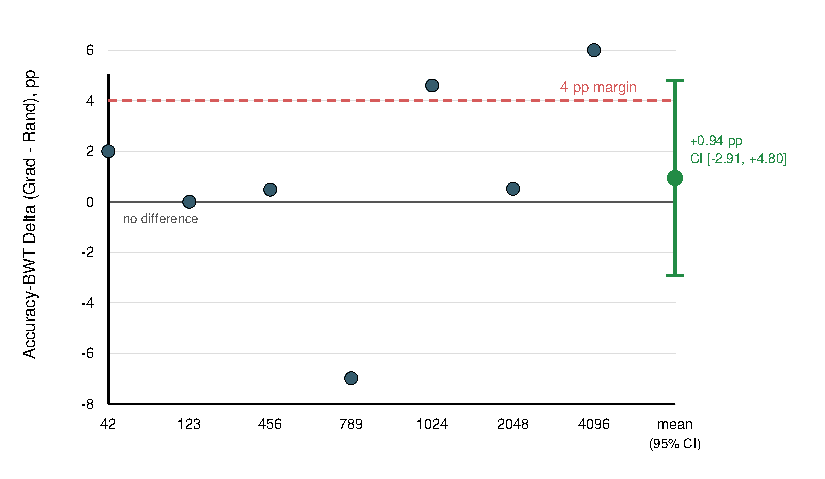
\includegraphics[width=0.6\textwidth]{figures/fig_accuracy_ci.pdf}
\caption{Accuracy-based validation. Blue points are the seven per-seed accuracy-BWT differences (Grad-B minus Random-B, percentage points) on the two discrete-option tasks, spanning $-6.98$ to $+6.00$ pp; green is the seven-seed mean with its 95\% interval $[-2.91,+4.80]$ pp. The plotted quantity is a difference of accuracy-BWT (mean final-minus-learned accuracy over prior tasks), a retention measure, not a difference of final accuracies. The interval spans zero, so no statistically reliable accuracy difference is detected, and it reaches past the 4 pp non-inferiority margin, so that criterion is not met. Per-seed values are in Appendix~\ref{app:accuracy_seeds}.}
\label{fig:accuracy_ci}
\end{figure}

Loss-based BWT is a proxy for forgetting rather than the quantity of ultimate interest, so we evaluate
the same masking comparison on task accuracy and ask whether the accuracy ordering agrees with
the loss ordering. The evaluation reuses the primary protocol and the corrected task evaluators over
the same seven seeds and 100 evaluation items per task, retraining from the base model on an A800
rather than re-scoring a checkpoint. Accuracy is scored only for the two tasks with discrete options
(Medical, MedQA four options; Legal, CaseHOLD), so every quantity below concerns those two.

Across seven seeds, the accuracy-BWT difference averages $+0.94$ percentage points with a
95\% interval of $[-2.91,+4.80]$ pp that spans zero. Here accuracy-BWT is the mean
final-minus-learned accuracy over the prior discrete-option tasks, so it measures retention on the
same footing as loss-based BWT and is not a difference of final accuracies. The individual seeds
range from $-6.98$ to $+6.00$ pp, and it is that spread rather than a large mean that makes the
interval wide at $n=7$. A 4 pp non-inferiority margin was specified in advance, and the measured
upper bound exceeds it, so non-inferiority is not established.

On the loss side, the same masks are separated: Grad-B forgets more in all seven seeds by a mean
of $+0.152$ on the A800 loss runs. This agrees in mean to within $0.003$ with the V100 estimate
after aligning sign conventions ($+0.155$ under [Grad $-$ Random]). Loss therefore resolves a
difference the accuracy measurement does not; the accuracy interval bounds that difference rather
than contradicting it.

Per-seed values and the interval construction are reported in Appendix~\ref{app:accuracy_seeds}.
Math is excluded from the accuracy read-out because its generation-based score is confounded by
truncation (Appendix~\ref{app:math_audit}).

